\section{Experiments}
\label{sec:experiments}

\paragraph{Protocol.} Every comparison changes one knob of a base configuration; a run refuses to start if its
configuration differs from the declared change. Predictions and falsification criteria are committed before any run,
and verdicts (pass / fail / inconclusive) are computed from those committed rules only. All arms share seeds
(five per experiment), probe inputs and the learning rate, which is fixed once on an unconditional run. Intervals are
95\% paired bootstrap CIs over seeds. Every experiment also trains the original Drifting objective, unchanged, as a
reference that is reported but not judged.

\subsection{Fixed points in a particle system}
\label{sec:l0}

Without a network, each of 32 conditions on a line owns 256 particles moved by $x \leftarrow x + \eta V(x\mid c)$, \ie
a generator of unlimited capacity, with one positive per condition. The field matches the autograd score ratio of
Lemma~\ref{lem:score} to \EZeroOneErr\ (float64; \VerdictEZeroOne). Increasing $h_q$ from $0$ to $h_p$ moves the
equilibrium monotonically from the mixture to memorisation (\cref{fig:l0}; \VerdictEZeroFour), whereas the original
Drifting objective memorises outright (own-positive share \EZeroThreeDriftingSelf).

\begin{figure*}[t]
  \centering
  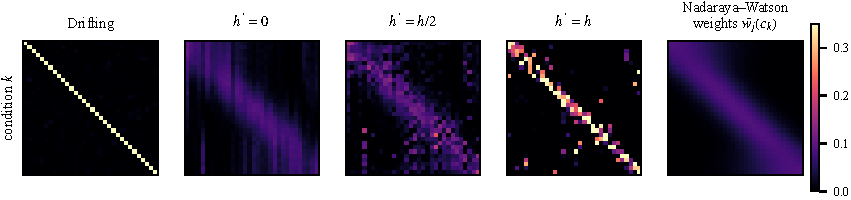
\includegraphics[width=\linewidth]{generated/figures/fig_l0}
  \caption{\textbf{$h_q$ selects the equilibrium} (particles, seed mean). Share of each condition's particles
  nearest to each positive. Original Drifting memorises (diagonal). \affd with $h_q=0$ spreads mass over the
  borrowed neighbours, as the Nadaraya--Watson weights $\tilde w$ predict (right); larger $h_q$ narrows the band
  toward memorisation.}
  \label{fig:l0}
\end{figure*}

The point-level assignment, however, misses the pre-registered tolerance for the mixture
(TV \EZeroThreeTV\ against $0.1$; \VerdictEZeroThree): with a kernel wider than the spacing of the positives, the
field cannot resolve which nearby positive a particle sits on. Compared at the kernel's resolution --- TV between the
$\sigma$-smoothed densities, an analysis we did not pre-register --- the equilibrium matches $\hat p$ to
\EZeroThreeSmoothTV. A counterfactual negative between two conditions has the predicted closed-form Gaussian
equilibrium in its algebra (relative error \EZeroFiveBMaxErr\ under a Gaussian closure), but with finite samples it is
stable only for small weights (error \EZeroFiveLamQuarterErr\ at $\lambda=0.25$, divergence from $\lambda=0.5$;
\VerdictEZeroFive).

\subsection{Mean collapse and its repair in a 2-D toy}
\label{sec:l1}

\paragraph{Setup.} Conditions $c\in[0,1]^2$ are drawn once; each of the $10{,}000$ training conditions has a single
positive from $p(x\mid c)$, a three-mode Gaussian mixture whose modes rotate with $c_1$ and whose radius and weights
change with $c_2$, so the conditional mean falls between modes. An MLP generator $f(\epsilon, g(c))$ sees $c$ quantised
to cells of width $\delta=1/16$, roughly 39 training conditions per cell. We train with Adam ($10^{-3}$, chosen on the
unconditional model: marginal $W_2$ \GFourCW\ against a sampling floor of \GFourCFloor), an EMA of the weights,
$20{,}000$ steps, and 8 conditions $\times$ 64 samples per batch, and evaluate on 256 held-out conditions with 512
samples each. The mean-collapse index is $\mathrm{MCI} = 1 - \operatorname{tr}\mathrm{Cov}_q/\operatorname{tr}\mathrm{Cov}_p$.

\paragraph{Single positive collapses (C1).} Both the original Drifting objective and the single-positive objective
collapse every condition to a point at the conditional mean (MCI \EOneTwoDriftingMCI\ and \EOneTwoSingleMCI;
off-manifold share \EOneTwoSingleOff), while the oracle with 16 true samples per condition and step covers the modes
(MCI \EOneTwoOracleMCI, mode coverage \EOneTwoOracleCov). This is the failure \affd targets
(\VerdictEOneTwo).

\begin{table}[t]
  \centering
  \small
  \resizebox{\linewidth}{!}{% generated — do not edit
\begin{tabular}{@{}lccccc@{}}
\toprule
Method & $W_2$ $\downarrow$ & $\operatorname{tr}\Sigma_q/\operatorname{tr}\Sigma_p$ & Prec. $\uparrow$ & Rec. $\uparrow$ & Modes $\uparrow$ \\
\midrule
Drifting & $1.4$ & $2.8\times10^{-5}$ & $0.0023$ & $0$ & $0.34$ \\
One positive ($h\to 0$) & $1.4$ & $3.8\times10^{-4}$ & $0.0017$ & $1.5\times10^{-6}$ & $0.35$ \\
Constant sample kernel & $1.3$ & $0.012$ & $0.0022$ & $0.007$ & $0.48$ \\
Random neighbors & $1.1$ & $1.3$ & $0.1$ & $0.97$ & $1$ \\
Noisy positive & $1.4$ & $4.4\times10^{-4}$ & $1.2\times10^{-5}$ & $0$ & $0.36$ \\
\midrule
\textbf{Affinity Drifting} & $0.47$ & $0.97$ & $0.74$ & $0.94$ & $1$ \\
Oracle (16 samples) & $0.5$ & $0.91$ & $0.83$ & $0.78$ & $0.98$ \\
\bottomrule
\end{tabular}
}
  \caption{\textbf{2-D toy, held-out conditions} (seed means). Above the line: the single-positive regime and the
  three mechanism controls; below: the oracle upper bound. [pending] entries fill in when E1.3 is aggregated.}
  \label{tab:l1}
\end{table}

\paragraph{Borrowing restores the mixture (C2).} \affd against the single-positive objective and controls K1--K3 is
\VerdictEOneThree\ (held-out $W_2$: \affd \EOneThreeAffDW, single \EOneThreeSingleW, ratio \EOneThreeRatio;
\cref{tab:l1}). \Cref{fig:mechanism} shows the mechanism: with one positive every attraction arrow points at the same
target, whereas the borrowed positives split the space into one basin per mode.

\begin{figure}[t]
  \centering
  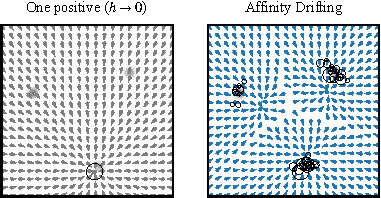
\includegraphics[width=\linewidth]{generated/figures/fig_mechanism}
  \caption{\textbf{Mechanism.} Direction of the attraction $\Vp(x\mid c)$ for one training condition. Single
  positive: every arrow points at the one target. \affd: arrows point to the nearest mode of the borrowed positives
  (circles, size $\propto$ weight).}
  \label{fig:mechanism}
\end{figure}

\paragraph{The gap grows with lost capacity (C3).} \VerdictEOneFour\ (\cref{fig:phase}).

\begin{figure}[t]
  \centering
  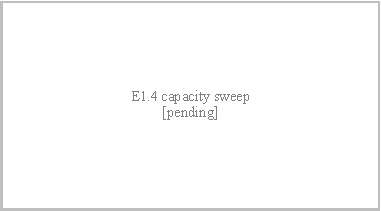
\includegraphics[width=\linewidth]{generated/figures/fig_phase}
  \caption{\textbf{Capacity.} $W_2$ of the single-positive objective and of \affd as the generator's resolution in
  $c$ coarsens (seed mean, 95\% CI).}
  \label{fig:phase}
\end{figure}
